\documentclass[10pt,border=0pt]{standalone}
% Shared by every standalone figure in this folder. Each figure is built once
% (make figures) and the same PDF is used by the report and, exported as PNG,
% by the README. Times text and 10pt sizes match IEEEtran, so the report
% includes each PDF at its natural size and no font is rescaled. Every
% picture draws its own white background of exactly the width it is placed
% at: 252pt for one column, 516pt for both.
\usepackage{mathptmx}
\usepackage{tikz}
\usetikzlibrary{arrows.meta,positioning,calc,fit,backgrounds}
\usepackage{pgfplots}
\pgfplotsset{compat=1.18}
\usepgfplotslibrary{groupplots}
% Reproducible bytes: no dates or random ids in the PDF.
\pdfinfoomitdate=1
\pdftrailerid{}
\pdfsuppressptexinfo=-1
\newlength{\colw}\setlength{\colw}{252pt}
\newlength{\textw}\setlength{\textw}{516pt}
\tikzset{
  every node/.style={font=\footnotesize},
  line/.style={draw=black!70, line width=0.6pt},
  arr/.style={line, -{Latex[length=4pt,width=3.4pt]}},
  box/.style={draw=black!55, line width=0.5pt, rounded corners=2pt, align=center,
    inner sep=2.5pt, minimum height=22pt},
  exec/.style={box, fill=blue!7},
  stage/.style={box, fill=orange!10},
  eval/.style={box, fill=green!9},
  store/.style={box, fill=black!7, rounded corners=0pt},
  note/.style={font=\scriptsize\itshape, text=black!75, align=center,
    execute at begin node={\hyphenpenalty=10000\exhyphenpenalty=10000}},
  frame/.style={draw=black!45, dashed, line width=0.5pt, rounded corners=3pt},
}
\newcommand{\figbackground}[2]{%
  \fill[white] (0,0) rectangle (#1,-#2);
  \useasboundingbox (0,0) rectangle (#1,-#2);}

% End-to-end architecture, drawn from the code:
%   runner      src/aire/runner/async_runner.py (worker pool, asyncio.timeout,
%               store.append_trace for each finished case)
%   ModelClient src/aire/providers/client.py, in the order complete() applies
%               them: quota circuit, cache, single flight, limiter, retries
%   limiter     src/aire/providers/ratelimit.py (RPM and TPM buckets, AIMD)
%   adapters    src/aire/providers/{local,openai_sdk,anthropic_sdk,gemini_sdk}.py
%   telemetry   src/aire/telemetry/ (aire otel-export, aire otel-ingest)
%   gate        src/aire/regression/compare.py, gate.py; src/aire/ci/pr_check.py
\begin{document}
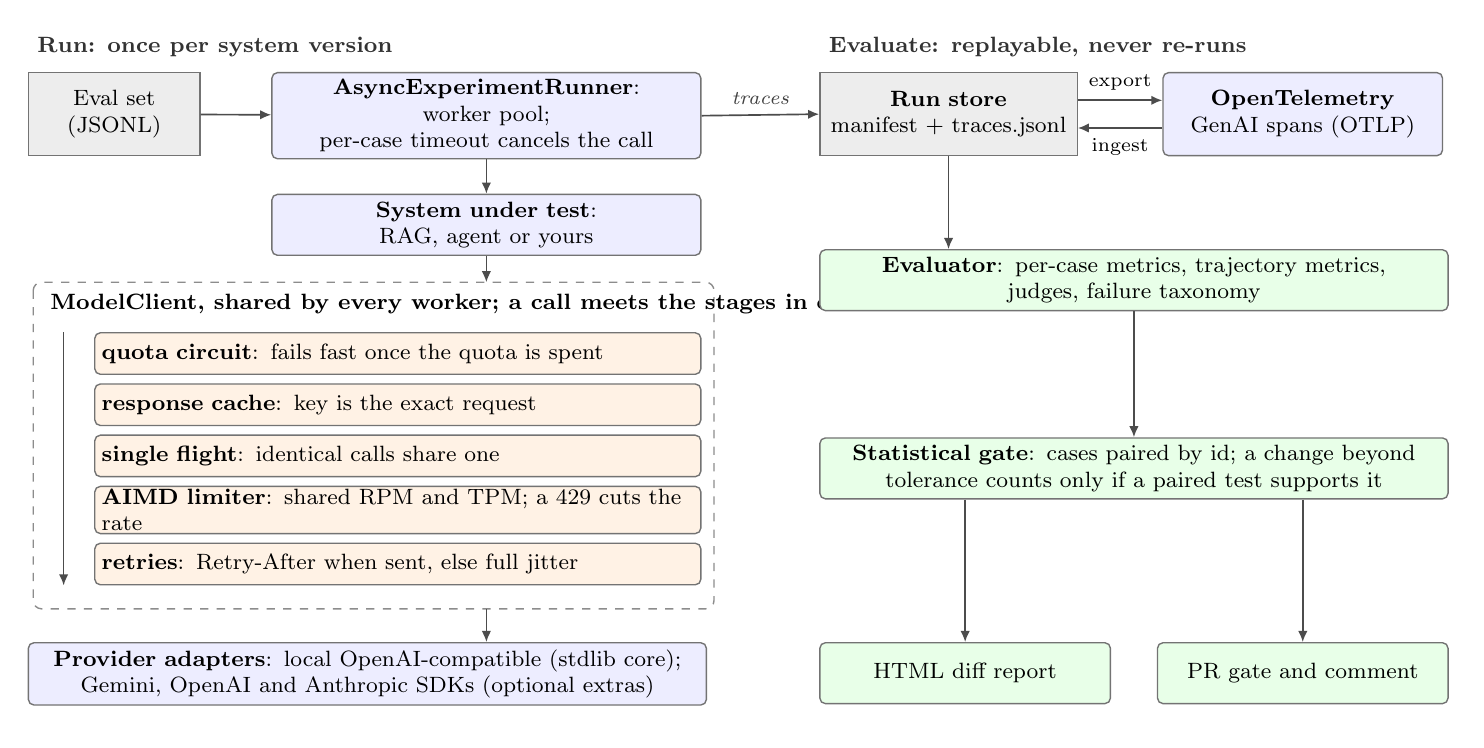
\begin{tikzpicture}[x=1pt,y=1pt]
\figbackground{516}{250}
\tikzset{
  head/.style={font=\footnotesize\bfseries, text=black!80},
  row/.style={stage, minimum height=15pt, inner ysep=1pt, text width=214pt, align=left,
    anchor=north west},
}
\node[head, anchor=north west] at (0,0) {Run: once per system version};
\node[head, anchor=north west] at (286,0) {Evaluate: replayable, never re-runs};

% Left column: the run path
\node[store, minimum width=62pt, minimum height=30pt, anchor=north west] (data) at (0,-16)
  {Eval set\\(JSONL)};
\node[exec, text width=150pt, minimum height=30pt, anchor=north west] (runner) at (88,-16)
  {\textbf{AsyncExperimentRunner}: worker pool;\\per-case timeout cancels the call};
\node[exec, text width=150pt, anchor=north west] (sut) at (88,-60)
  {\textbf{System under test}: RAG, agent or yours};
\draw[arr] (data) -- (runner);
\draw[arr] (runner) -- (sut);

\node[row] (q) at (24,-110) {\textbf{quota circuit}: fails fast once the quota is spent};
\node[row, below=3pt of q] (c) {\textbf{response cache}: key is the exact request};
\node[row, below=3pt of c] (f) {\textbf{single flight}: identical calls share one};
\node[row, below=3pt of f] (l) {\textbf{AIMD limiter}: shared RPM and TPM; a 429 cuts the rate};
\node[row, below=3pt of l] (r) {\textbf{retries}: Retry-After when sent, else full jitter};
\draw[frame] (2,-92) rectangle (248,-210);
\node[anchor=north west, inner sep=0pt, font=\footnotesize\bfseries] at (8,-96)
  {ModelClient, shared by every worker; a call meets the stages in order};
\draw[arr] ($(q.north west) + (-11,0)$) -- ($(r.south west) + (-11,0)$);
\draw[arr] (sut.south) -- (sut.south |- 0,-92);
\node[exec, text width=240pt, anchor=north west] (adapt) at (0,-222)
  {\textbf{Provider adapters}: local OpenAI-compatible (stdlib core);\
   Gemini, OpenAI and Anthropic SDKs (optional extras)};
\draw[arr] (sut.south |- 0,-210) -- (adapt.north -| sut.south);

% Right column: evaluation over stored traces
\node[store, text width=88pt, minimum height=30pt, anchor=north west] (runs) at (286,-16)
  {\textbf{Run store}\\manifest + traces.jsonl};
\node[exec, text width=96pt, minimum height=30pt, anchor=north west] (otel) at (410,-16)
  {\textbf{OpenTelemetry}\\GenAI spans (OTLP)};
\draw[arr] ($(runs.east) + (0,5)$) -- ($(otel.west) + (0,5)$)
  node[midway, above, font=\scriptsize] {export};
\draw[arr] ($(otel.west) + (0,-5)$) -- ($(runs.east) + (0,-5)$)
  node[midway, below, font=\scriptsize] {ingest};
\draw[arr] (runner.east) -- (runs.west)
  node[midway, above, note] {traces};

\node[eval, text width=222pt, anchor=north west] (engine) at (286,-80)
  {\textbf{Evaluator}: per-case metrics, trajectory metrics,\\judges, failure taxonomy};
\node[eval, text width=222pt, anchor=north west] (gate) at (286,-148)
  {\textbf{Statistical gate}: cases paired by id; a change beyond\\
   tolerance counts only if a paired test supports it};
\node[eval, text width=100pt, anchor=north west] (html) at (286,-222)
  {HTML diff report};
\node[eval, text width=100pt, anchor=north west] (pr) at (408,-222)
  {PR gate and comment};
\draw[arr] (runs) -- (runs |- engine.north);
\draw[arr] (engine) -- (gate);
\draw[arr] (gate.south -| html) -- (html);
\draw[arr] (gate.south -| pr) -- (pr);
\end{tikzpicture}
\end{document}
